\chapter{Методы и их применение} \label{chap2}

\section{Имитация отжига}

\noindent
\textit{Имитация отжига} (\emph{Simulated Annealing}, SA) представляет собой алгоритм решения задачи по поиску глобального оптимума некоторой функции~$F\colon \mathbb{X} \to \mathbb{R}$ через упорядоченный стохастический поиск, базирующийся на моделировании физического процесса кристализации вещества из жидкого состояние в твердое.

ДОБАВИТЬ ВВЕДНИЕ

\subsection{Алгоритм}

\noindent Для описания метода рассмотрим задачу нахождения глобального минимума:
\[
	F(x) \to \min \limits _{x \in \mathbb{X}},
\]

\noindent где~$x = (x_{1},\ldots , x_{m})$~--- вектор всех состояний, $\mathbb{X}$~--- множество всех состояний.

Положим, что~$k = 0$~и изначально температура зафиксированна на определенном уровне~$T(k) = const$.


\begin{enumerate}
	\item  Из множества всех состояний выберем случайный элемент~$\widehat{x}(k) \equiv x_i$,

	$i \in (1, ..., m)$.

	\item Понизим температуру одним из следующих способов:

		\begin{enumerate}
			\item Больцмановский отжиг
			\begin{equation}
			T(k) =  \dfrac{T(0)}{\ln (1 + k)}, \ k > 0
			\label{eq:boltzman}
			\end{equation}

			\item Отжиг Коши
			\begin{equation}
			T(k)  =  \dfrac{T(0)}{k}
			\end{equation}

			\item Метод тушения
			\begin{equation}
			T(k+1) = \alpha T(k),\ \alpha \in (0, 1)
			\end{equation}

		\end{enumerate}


	\item Пусть следующий элемент зависит от функции из семейства симметричных вероятностных распределений $G:$~$ \mathbb{X} \to \mathbb{X}$, порождающей новое состояние:
	\[
	\tilde{x}(k) \thicksim G(\widehat{x}(k), T(k)).
	\]

	\begin{enumerate}

		\item Часто G выбирается из семейства нормальных распределений:
		\begin{equation}
		\label{eq:normal_G}
		G(\tilde{x}; \widehat{x}, T)
		=
		\dfrac{1}
		{\sqrt{(2\pi)^{D} T}}
		\exp
		\left\lbrace
		\dfrac{- |\tilde{x} - \widehat{x}|^2}{2T}
		\right\rbrace,
		\end{equation}

		где $\widehat{x}$ — математическое ожидание, $T$  — дисперсия, $D$ — размерность пространства всех состояний.

		\item Также для D = 1 используется распределение Коши с плотностью:
		\begin{equation}
		G(\tilde{x}; \widehat{x}, T)
		=
		\dfrac{1}{\pi}
		\dfrac{T}{|\tilde{x}- \widehat{x}|^2 + T^2},
		\end{equation}

		где~$\widehat{x}$~--- параметр сдвига, $T$~--- параметр масштаба.





	\end{enumerate}

	\item Рассчитываем разницу двух функций:
	\[
	\Delta F =
	F(\tilde{x}(k))
	-
	F(\widehat{x}(k)).
	\]

	\item Принимаем~$\tilde{x}(k)$~за новый элемент, то есть~$\widehat{x}(k+1) \equiv \tilde{x}(k)$, с вероятностью
	\begin{equation}
	\mathbb{P}(\{\widehat{x}(k+1) = \tilde{x}(k)\})
	=
	\begin{cases}
	1,
	&
	\Delta F <0
	\\
	\exp
	\left\lbrace
	- \dfrac {\Delta F}{T(k)}
	\right\rbrace ,
	&
	\Delta F \geqslant 0
	\end{cases}
	\end{equation}

	и отвергаем его, то есть~$\widehat{x}(k+1) \equiv \widehat{x}(k)$, с вероятностью
	\[
	q
	=
	1 - \mathbb{P}(\{\widehat{x}(k+1) = \tilde{x}(k)\}).
	\]

	Заметим, чем выше температура, тем больше вероятность принять состояние хуже текущего ($\Delta F \geqslant 0$).

	\item Возвращаемся к пункту 2, пока не достигнем глобального минимума.

\end{enumerate}


%%%%%%%%%%%%%%%%%%%%%%%%%%%%%%%%%%%%%%%%%%%%%%%%%%%%%%%%%%%%%%%%%%%%%%%%%%%%%%%%%%%%%%%%%%%%%


\subsection{N ферзей}
\noindent Рассмотрим задачу, в которой необходимо расставить $N$ ферзей на шахматной доске размера $N \times  N$ так, чтобы ни один из них не <<бил>> другого.

В таком случае, множество всех состояний $\mathbb{X}$ будет содержать всевозможные расстановки ферзей на шахмотной доске. Общее число возможных расположений $n$ ферзей на $N \times N$-клеточной доске равно:
\[
{\begin{pmatrix} N \times N  \\ n \end{pmatrix}} = \dfrac{N \times N!}{n! (N \times N - n)!}
\]

Тогда  функция~$F:$~$\mathbb{X} \to \mathbb{R}$ будет выдавать количество атак ферзей, и решением данной задачи будет нахождение такого распложения~$x^{*}$, что~$F(x^*) \equiv 0$.

Зафиксируем изначальное расположение ферзей на шахматной доске. Очевидно, что несколько ферзей не могут находиться на одной вертикали или горизонтали, ибо тогда они будут находиться под ударом друг-друга. Следовательно, наша задача сужается к поиску расположения:
\begin{equation}
x* = (q_1, ..., q_n) = \{(1, h_1), ..., (n, h_n)\}, h_1 \neq ...  \neq h_n,
\end{equation}

где $(i, h_i)$ — расположение ферзя $q_i$ на i-ой вертикали по горизонтали $h_i$.

Отметим, что такая задача имеет $N!$ решений.

\newgame
\fenboard{q7/1q6/2q5/3q4/4q3/5q2/6q1/7q w - - 0 1}

\begin{figure}[h!]
	\begin{center}
		\showboard
		\legend{}
		\caption{ --- Изначальное расположение.}
		\label{img:nonopt}
	\end{center}
\end{figure}

Определим функцию, которая будет создавать изначальное неоптимальное расположение, в общем виде. Учитем, что несколько ферзей не могут находиться на одной вертикали или горизонтали.

\begin{pyin}
def queens(N):
  ver = np.arange(1, N + 1)
  hor = np.arange(1, N + 1)
  np.random.shuffle(hor)
  return np.column_stack((ver, hor)) # получаем массив
  # размерности (N, 2), отождествляющий расположение ферзей
\end{pyin}

Выведем первоначальное расположение ферзей для стандартной доски $8 \times 8$, где первый столбец массива — расположение по вертикали, второй столбец массива — расположение по горизонтали. Для наглядности — презентации оптимизационного процесса — выстроим изначальную расстановку на главной диагонали (рис. \ref{img:nonopt}).


\begin{pyin}
matrix = queens(8)
matrix
\end{pyin}

\begin{pyout}
array([[1, 1],
       [2, 2],
       [3, 3],
       [4, 4],
       [5, 5],
       [6, 6],
       [7, 7],
       [8, 8]])
\end{pyout}


Функция F, которая выявляет количество атак ферзей, выглядит следующим образом:
\begin{pyin}
def F(Q, N):
  cnt = 0
  for i in range(N):
     for j in range(i + 1, N):
         if abs(Q[i, 0] - Q[j, 0]) == abs(Q[i, 1] - Q[j, 1]):
             cnt += 1
  return cnt * 2 # учитываем взаимные атаки
\end{pyin}

Посмотрим, сколько у атак у исходной расстановки.
\begin{pyin}
F(matrix, 8)
\end{pyin}

\begin{pyout}
56
\end{pyout}

В нашей задачи функция G будет случайной незначительной перестановкой номеров горизонтали в исходном наборе.

\begin{pyin}
def G(Q, N):
  pos = Q.copy()
  while True:
     i = np.random.randint(0, N - 1)
     j = np.random.randint(0, N - 1)
     if i != j:
        break
  pos[i, 1], pos[j, 1] = pos[j, 1], pos[i, 1]
  return pos # получаем новое расположение
\end{pyin}

Теперь выведем и сам метод имитации отжига.

\begin{pyin}
def SA(Q, T, schedule):
  N = np.shape(Q)[0]
  x_hat = Q.copy()
\end{pyin}

\begin{pyprint}
  while F(x_hat, N) != 0:
     x_tilda = G(x_hat, N)
     delta = F(x_tilda, N) - F(x_hat, N)
     prob = np.exp(- delta / T)
     if (delta < 0) or (prob >= np.random.random()):
        x_hat = x_tilda
     # используем метод тушения для понижения температуры
     T *= schedule
  return x_hat
\end{pyprint}


\newgame
\fenboard{2q5/4q3/1q6/7q/q7/6q1/3q4/5q2 w - - 0 1}

\begin{figure}[h!]
	\begin{center}
		\showboard
		\legend{}
		\caption[р]{ --- Оптимальное расположение}
		\label{img:opt}
	\end{center}
\end{figure}


Так для нашего примера с гиперпараметрами $T(0) = 100, \alpha = 0.9$ мы получаем следующее оптимальное решение (рис. \ref{img:opt}):

\begin{pyin}
SA(matrix, 100, 0.9)
\end{pyin}

\begin{pyout}
array([[1, 4],
       [2, 6],
       [3, 8],
       [4, 2],
       [5, 7],
       [6, 1],
       [7, 3],
       [8, 5]])
\end{pyout}

\begin{figure}[h!]
\centering
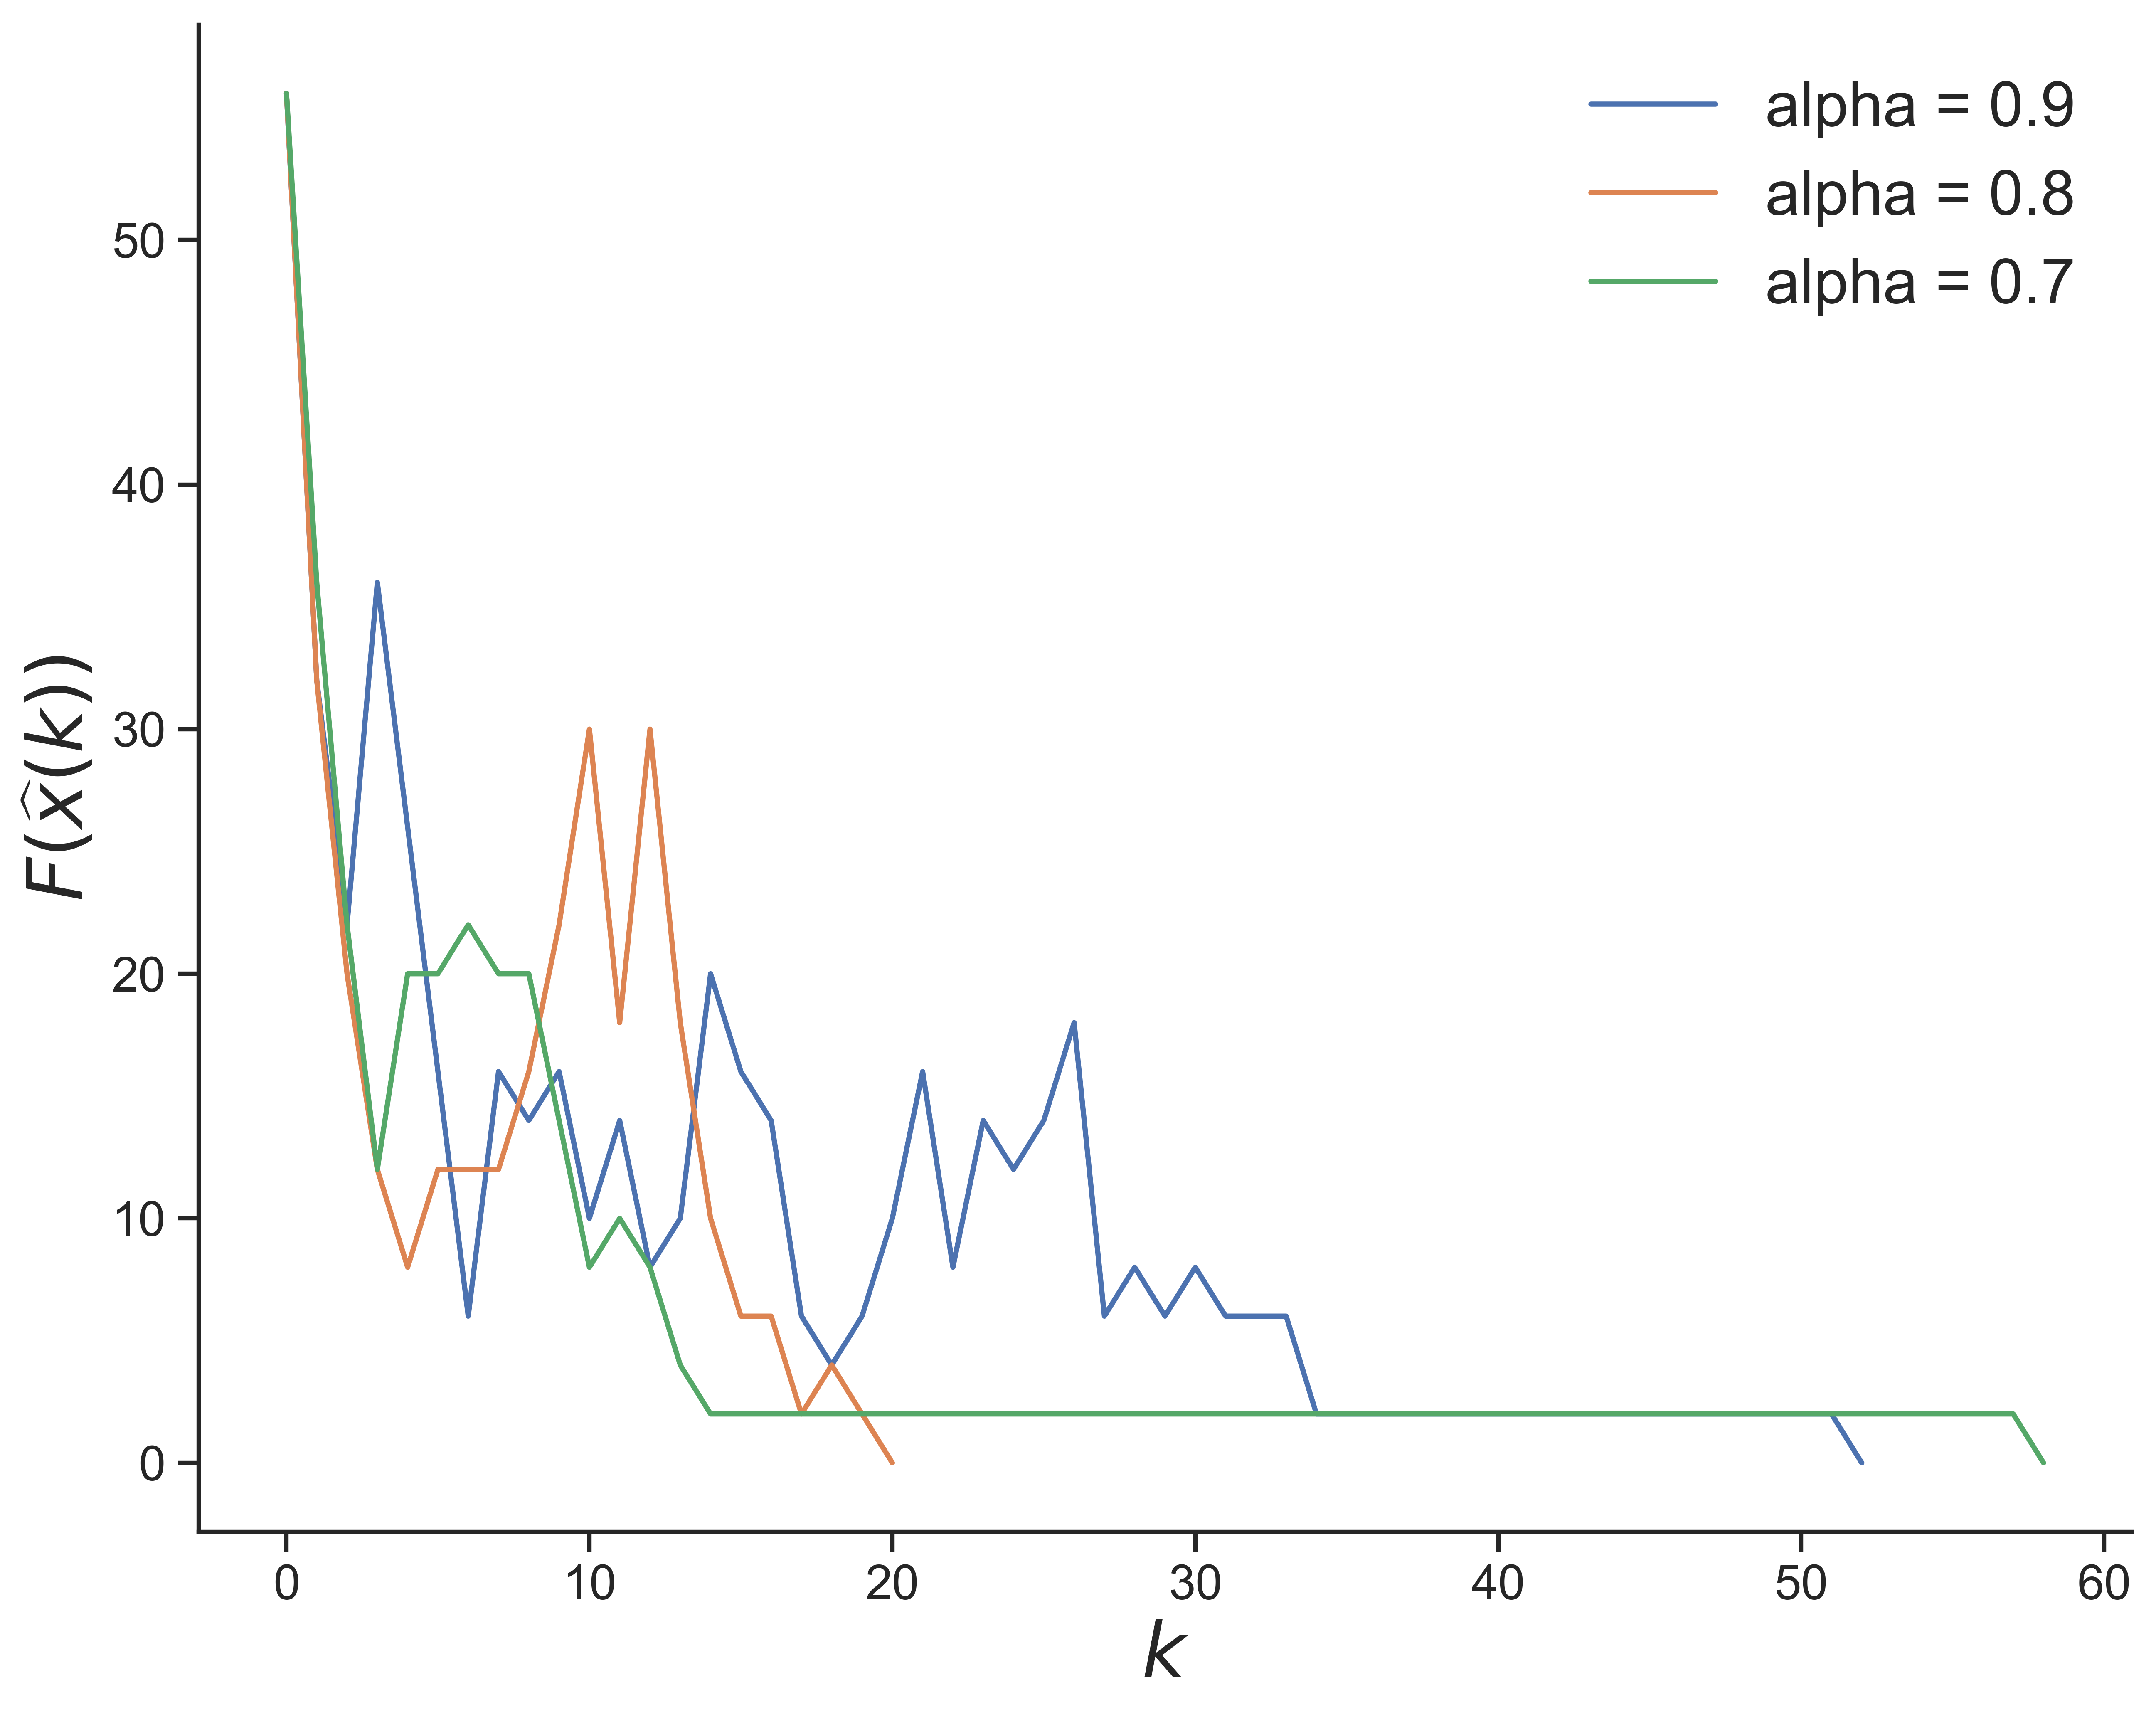
\includegraphics [width=120mm]{queens8}
\caption{ --- Оптимизация расстановки 8 ферзей  в зависимости от гиперпараметра $\alpha$.}
\label{img:queens8}
\end{figure}

\begin{figure}[h!]
\centering
\includegraphics [width=120mm]{queens25}
\caption{ --- Оптимизация расстановки 25 ферзей  в зависимости от гиперпараметра $\alpha$.}
\label{img:queens25}
\end{figure}

\newpage

%%%%%%%%%%%%%%%%%%%%%%%%%%%%%%%%%%%%%%%%%%%%%%%%%%%%%%%%%%%%%%%%%%%%%%%%%%%%%%%%%%%%%%%%%%%%%


\subsection{Минимизация негладкой функции}

\noindent Воспользуемся алгоритмом имитации отжига для нахождения глобального минимума следующей функции:
\[
f(x) = x^2 (1 + |\sin 80x|).
\]

	\begin{figure}[h]
	\centering
	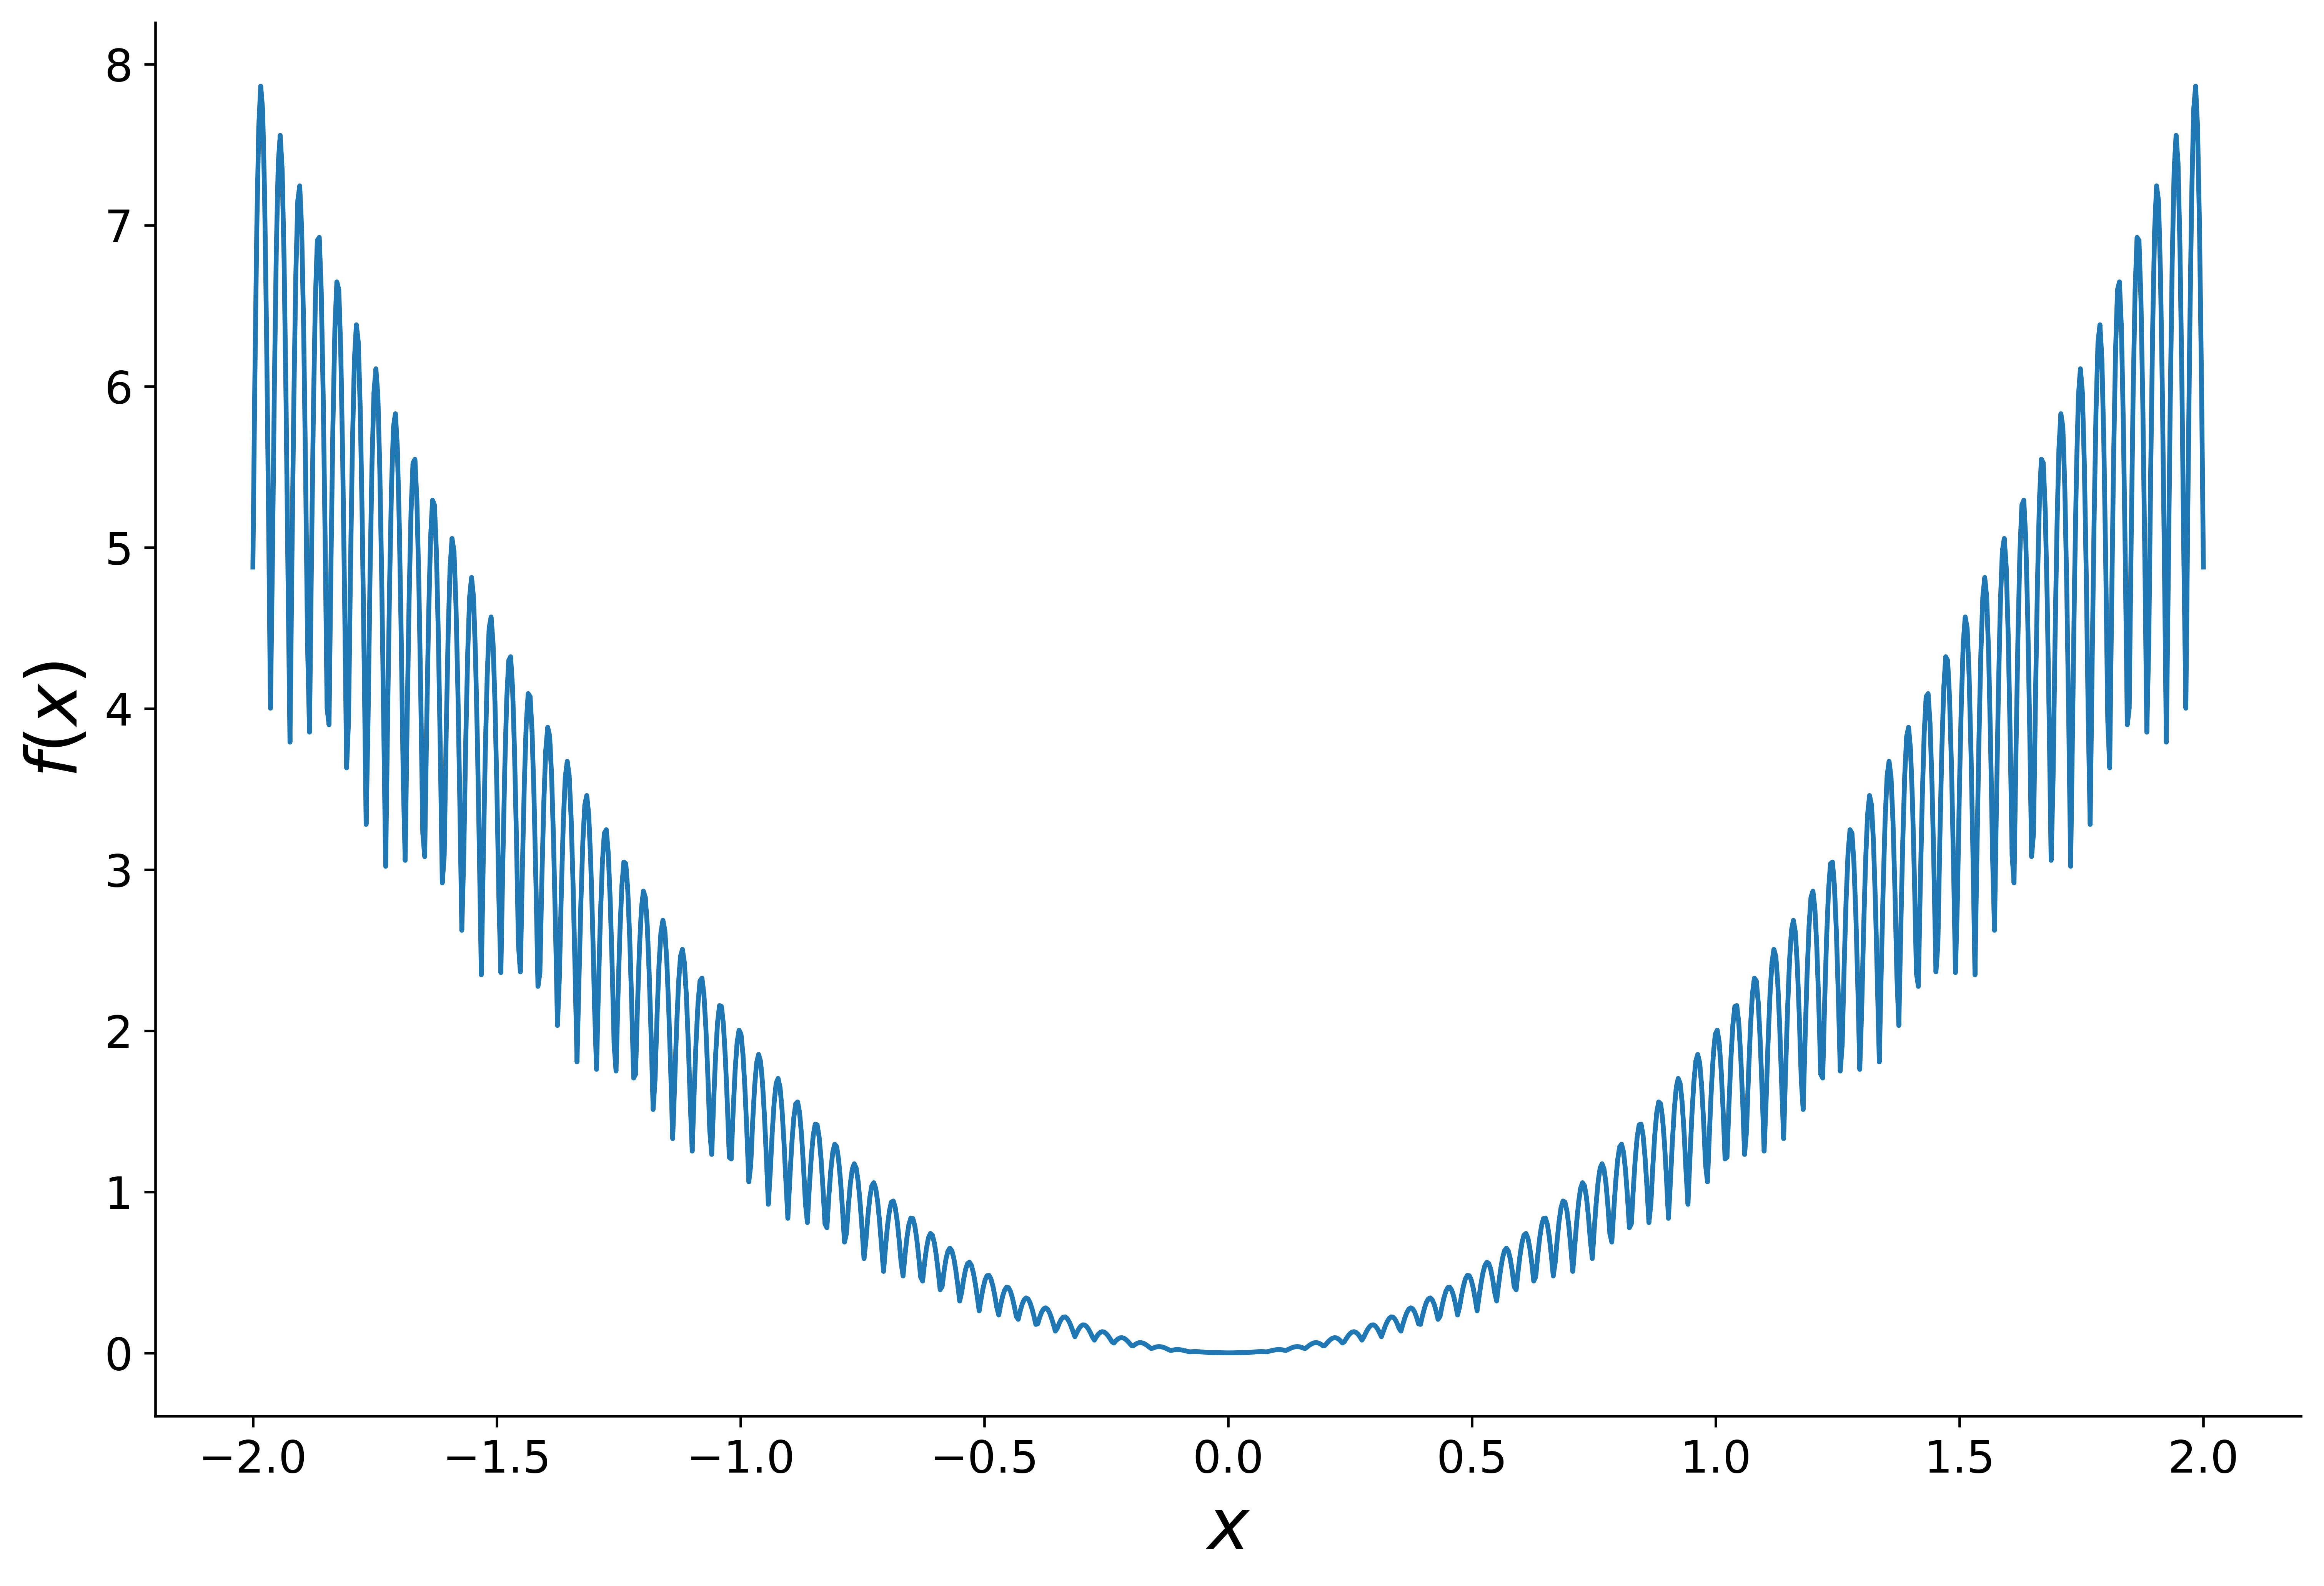
\includegraphics[width=120mm]{func_min}
	\caption{}
	\label{img:func_min}
\end{figure}

Стандартные методы оптимизации --- к примеру, метод градиентного спуска --- в данном случае не применимы. Вследствие наличия модуля этп функция не дифференцируема. Также она имеет очень большое количество локальных минимумов, что затрудняет, к примеру, мультистарт --- запуск градиентного спуска из разных начальных направлений.

Применим наш алгоритм к данной задачи. Пусть~$T(0) = 0.6$. Для понижения температуры будем использовать Больцмановский отжиг~(\ref{eq:boltzman}), а в качестве функции вероятностных распределений $G$ — семейство нормальных распределений~(\ref{eq:normal_G}).

\begin{pyin}
def SA(space, T, epsilon): # за space берется np.linspace(-2,2,1000)
  x_hat = np.random.choice(space)
  T_0 = T
  k = 1
  while True:
     x_tilda = np.random.normal(x_hat, T)
     delta = F(x_tilda) - F(x_hat)
     prob = np.exp(- delta / T)
\end{pyin}

\begin{pyprint}
     if (delta < 0) or (prob >= np.random.random()):
        x_hat = x_tilda
     if (x_hat < epsilon) and (x_hat > 0):
        return x_hat
     T = T_0 / np.log(1 + k)
     k += 1
\end{pyprint}

Остановка итерационного процесса и скорость метода зависят от того, насколько близко мы хотим приблизиться к глобальному минимуму. Так, при точности~$10^{-1}$, что довольно много, для 1000 повторений алгоритма метод отжига находит глобальный минимум в среднем за~1.97e-3~секунды со стандартным отклонением в~3.47e-5~секунды. Однако, увеличив точность до~$10^{-6}$, среднюю скорость занимает уже~1.27~секунды со стандартным отклонением в~2.1e-5~секунды. Это наглядно представлено на рисунке \ref{img:func_min1}.

\begin{figure}[h!]
	\centering
	\includegraphics[width=\linewidth]{func_min1}
	\caption{ --- Оптимизационный процесс в зависимости от точности.}
	\label{img:func_min1}
\end{figure}

\newpage

\subsection{Задача коммивояжера}

\noindent \emph{Задача коммивояжера} (\emph{Traveling Salesman Problem}, TSP) является образцовым методом проверки многих оптимизационных алгоритмов и заключается в поиске кратчайшего маршрута между городами. Путь должен быть проложен так, чтобы маршрут единственно проходил через все города и его конечная точка совпадала с  изначальной.

TSP имеет множество приложений в планировании и логистике, а также выступает в качестве подзадачи во многих других областях.  В таком случае города могут представлять, к примеру, клиентов, а расстояние между городами — время или стоимость путешествия.

\begin{figure}[h!]
\centering
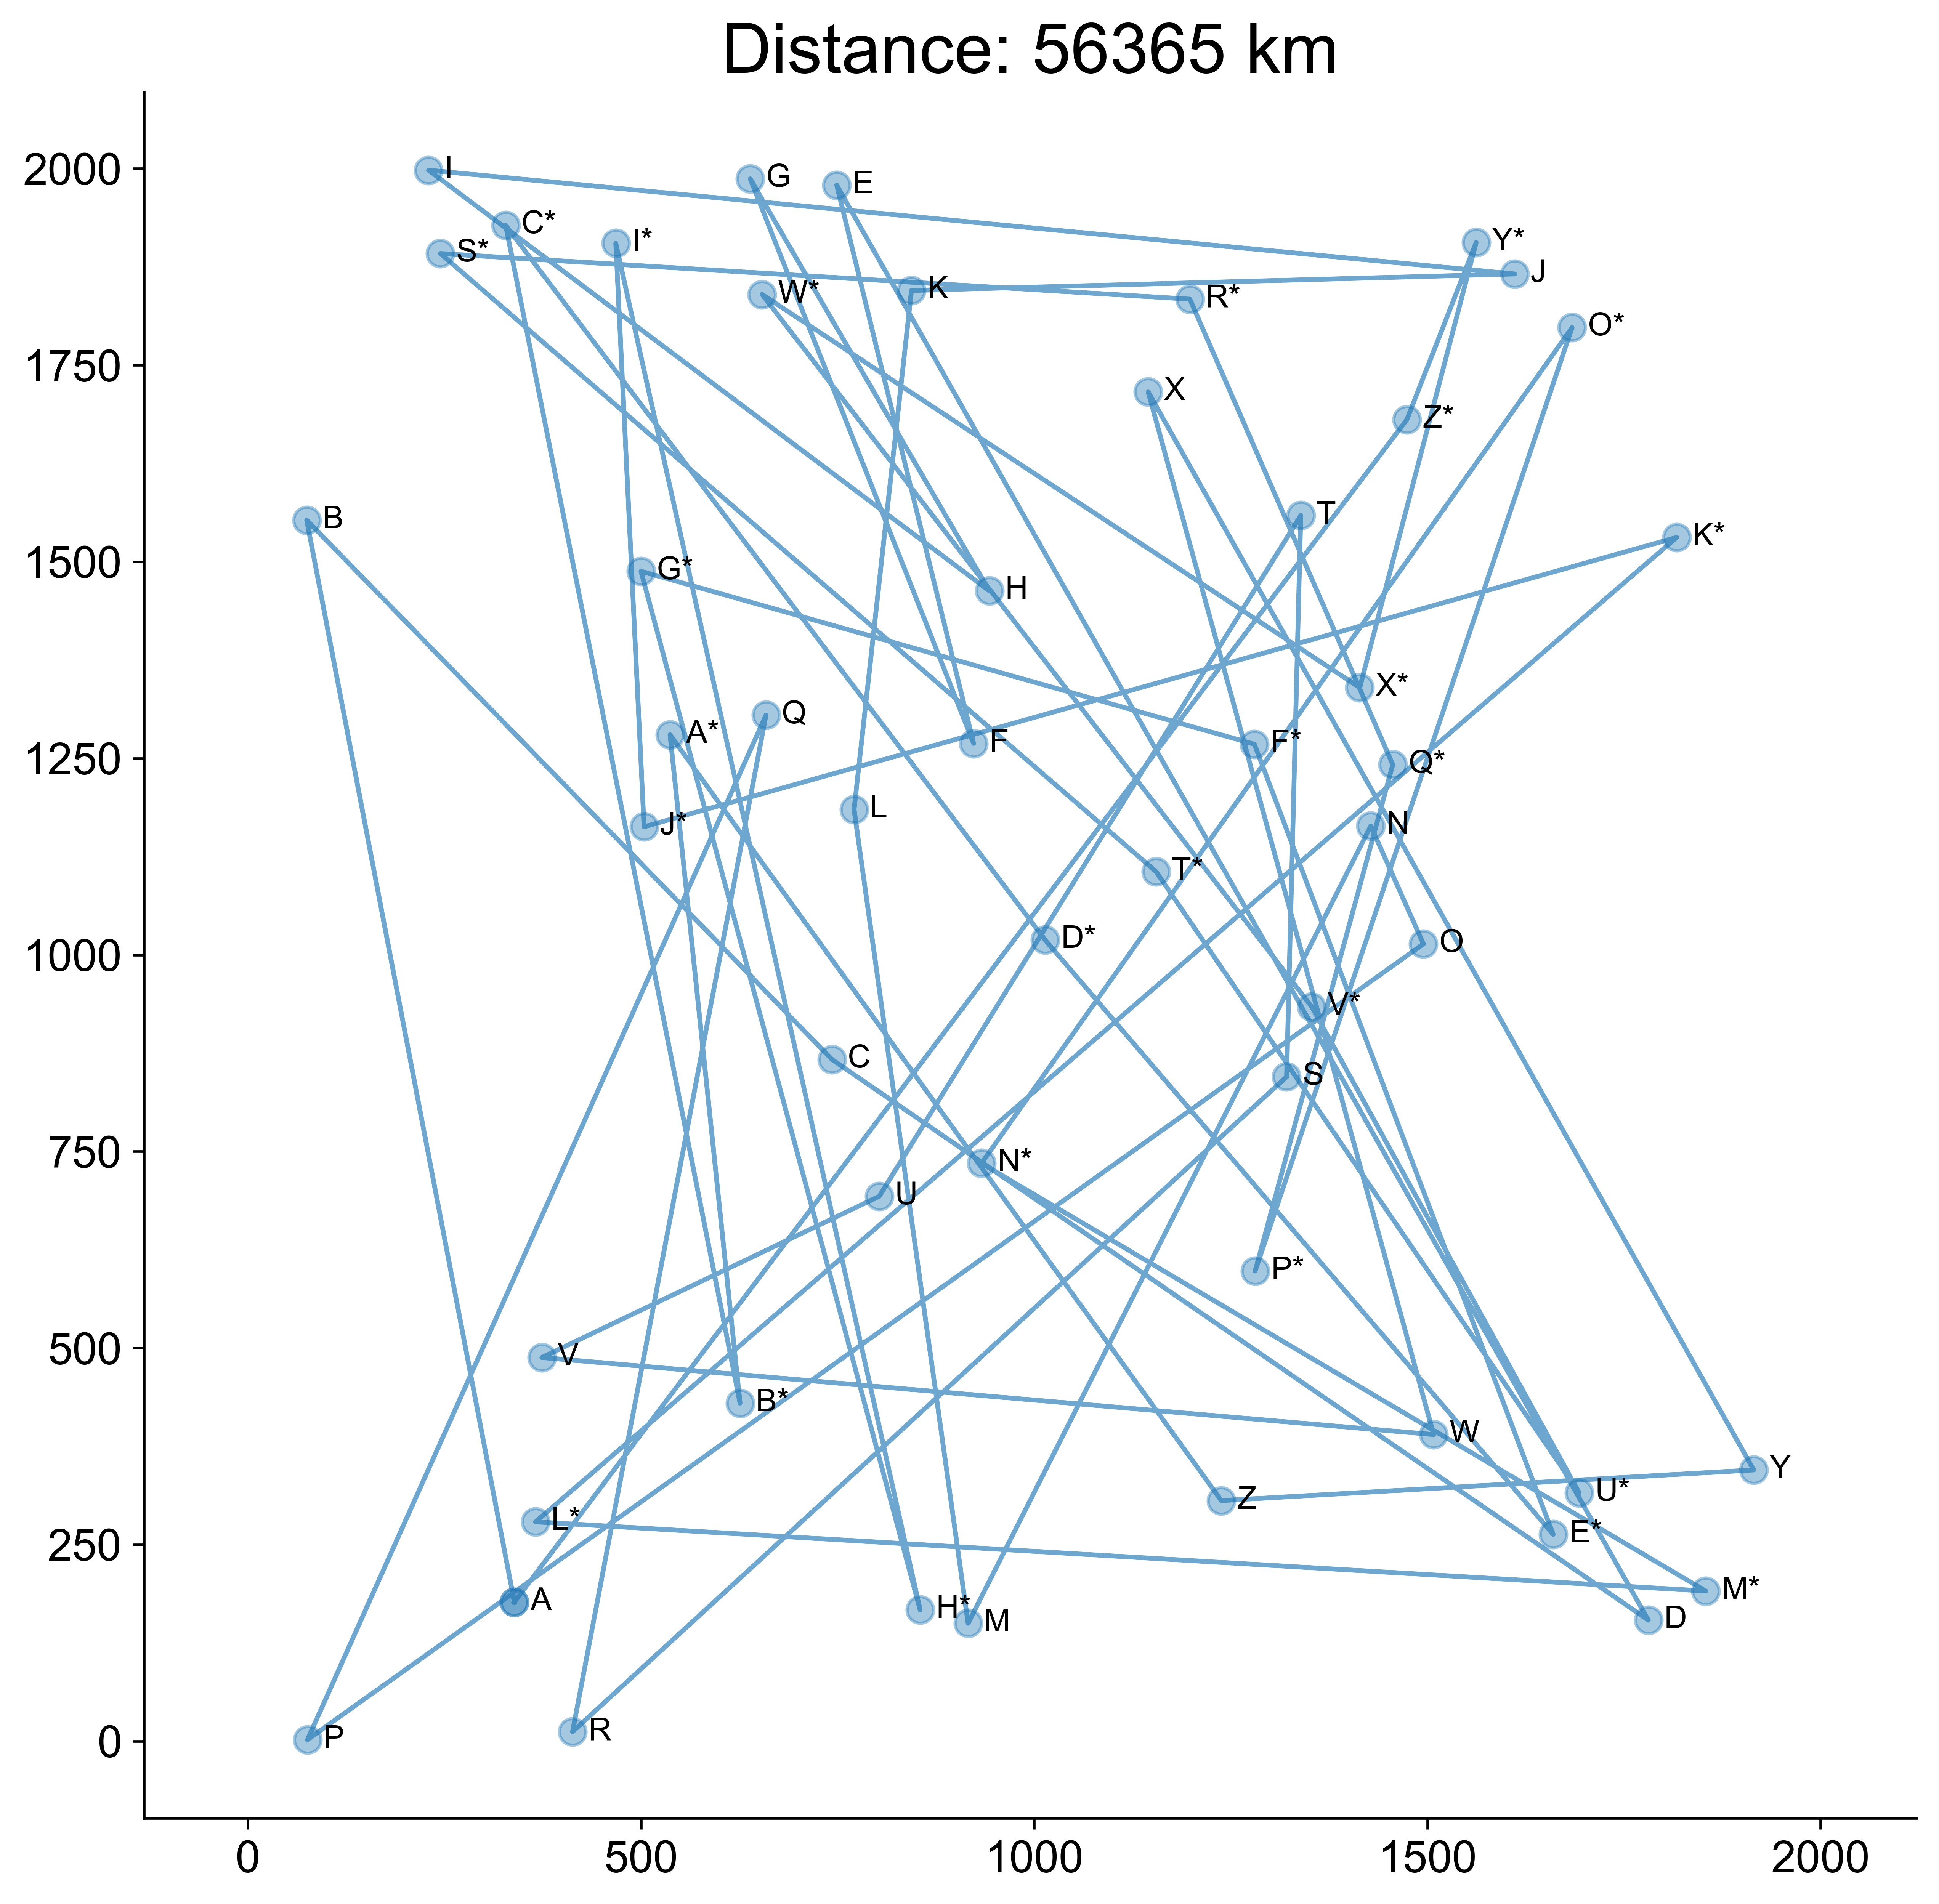
\includegraphics [width=120mm]{TSP1}
\caption{ --- Изначальный маршрут для 26-ти городов.}
\label{img:tsp1}
\end{figure}

Для нашего примера создадим карту. Функция map\_city будет принимать желаемое количество городов в качестве входных данных и выдавать два списка, из которых далее создается общий список кортежей. Первым элементом кортежа является наименование города, а вторым --- его расположение в декартовой системе координат.

\begin{pyin}
def map_city(cities_num):
  letters = [chr(i) for i in range(65, 65 + cities_num)]
  coord = np.random.randint(1, 500, size=(cities_num, 2))
  return letters, coord
\end{pyin}

Наш маршрут будет состоять из 26-ти городов.

\begin{pyin}
names, cities = map_city(26)
store_val = list(zip(names, cities))
\end{pyin}


Определим расстояние от города i до всех остальных посредством функции distance\_dict. Для измерения расстояния между городами будем использовать евклидову метрику. Напомним, что евклидово расстояние между точками~$x = (x_1, ..., x_d)$~и~$u = (u_1, ..., u_d)$~задается как:
\[
d (x, u)
=
\sqrt{
\sum_{i = 1}^d \limits
(x_i - u_i)^2
}
\]

\begin{pyin}
def distance_dict(cities, n):
  d = dict()
  for i in range(n):
     city = dict()
     for j in range(n):
        if i == j:
           continue
        c_a = cities[i][1]
        c_b = cities[j][1]
        dist = np.sqrt((c_a[0] - c_b[0])**2 + (c_a[1] - c_b[1])**2)
        city[cities[j][0]] = dist
     d[cities[i][0]] = city
  return d
\end{pyin}


\begin{pyin}
cities_d = distance_dict(store_val, len(store_val))
\end{pyin}


Функция F для подсчета общего расстояния путешествия:

\begin{pyin}
def F(path, cities):
  dist = 0
  for i in range(len(path) - 1):
     dist += cities[path[i]][path[i + 1]]
  dist += cities[path[i + 1]][path[0]]
  return dist
\end{pyin}

За функцию G будет выступать простая перестановка как и в задаче о N ферзях.

\begin{pyin}
def G(path, n):
  pos = path.copy()
  while True:
     i = np.random.randint(0, n - 1)
     j = np.random.randint(0, n - 1)
     if i != j:
        break
     pos[i], pos[j] = pos[j], pos[i]
  return pos
\end{pyin}

\begin{figure}[h!]
\centering
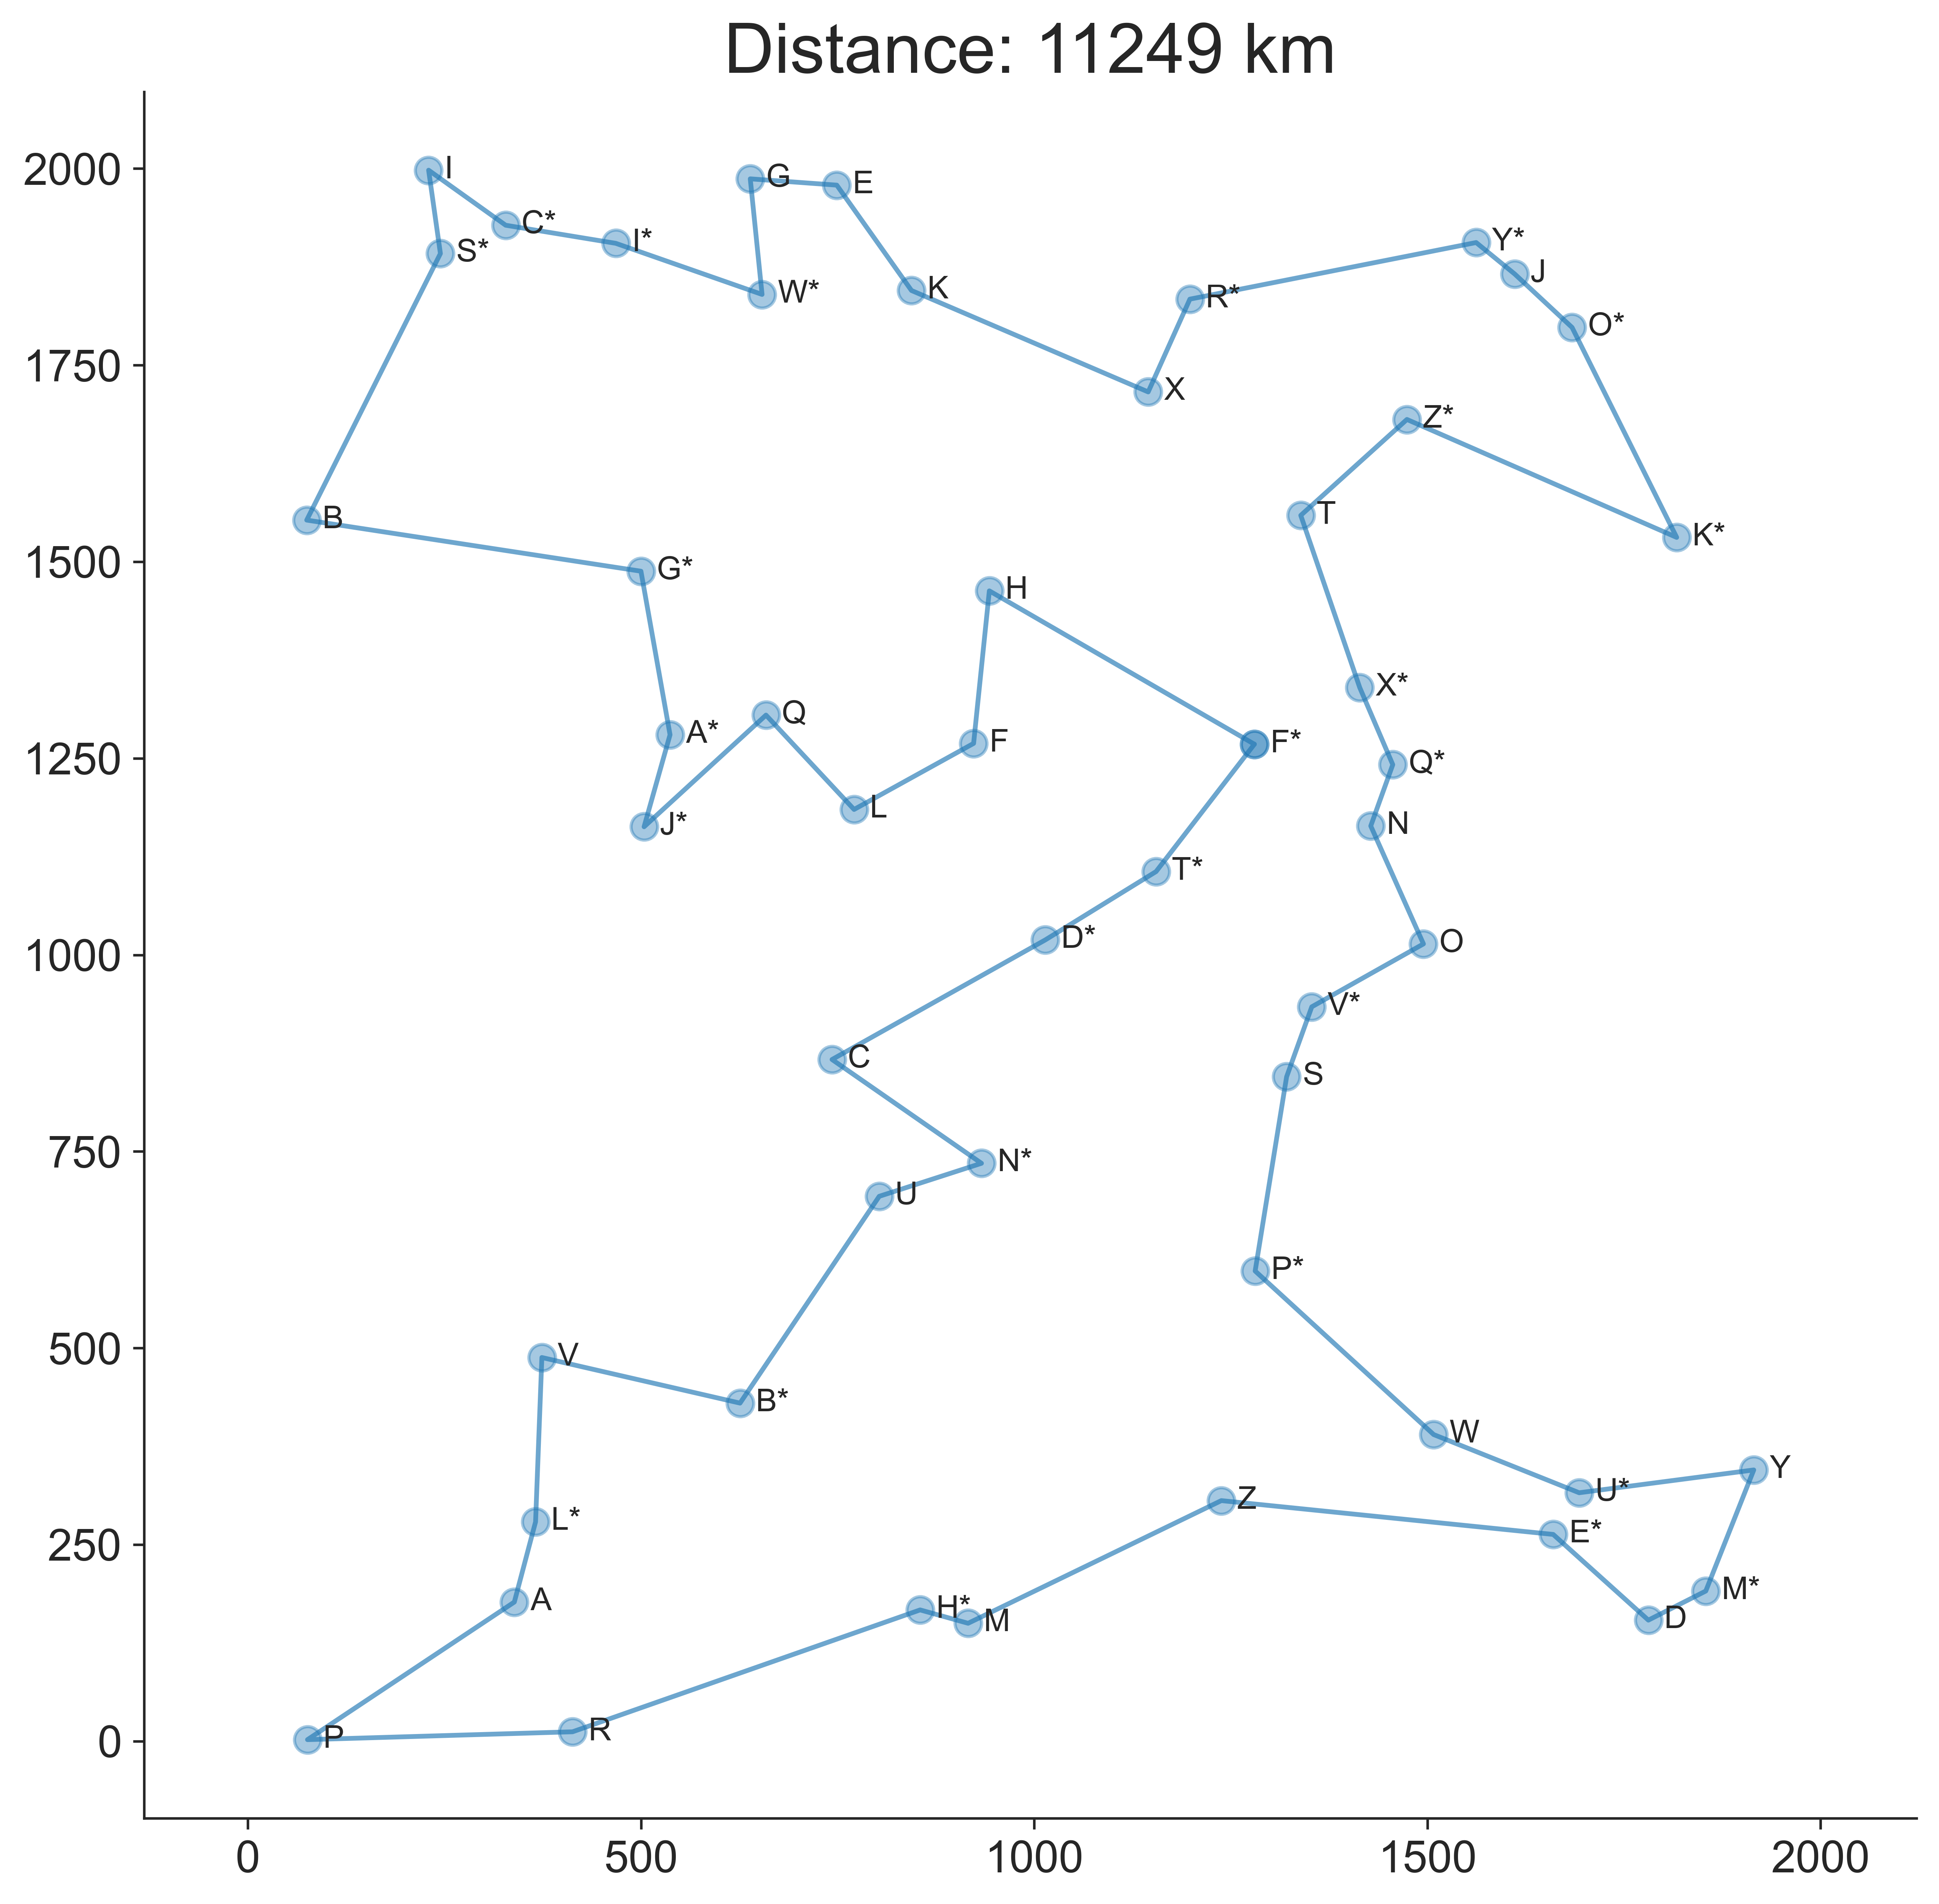
\includegraphics [width=120mm]{TSP2}
\caption{ --- Применение метода отжига для построения оптимального маршрута для 26-ти городов.}
\label{img:tsp2}
\end{figure}


Для понижения температуры используем Больцмановский отжиг~(\ref{eq:boltzman}).

\begin{pyin}
def SA(path, T):
  path_hat = path
  n = len(path_hat)
  np.random.shuffle(path_hat)
  T_0 = T
  k = 1
  for i in range(100000):
     path_tilda = G(path_hat, n)
     delta = F(path_tilda, cities_d) - F(path_hat, cities_d)
\end{pyin}

\begin{pyprint}
     prob = np.exp(- delta / T)
\end{pyprint}

Теперь построим оптимальный маршрут (рис.~\ref{img:tsp2}).

\begin{pyin}
path_opt = SA(names, 100)
\end{pyin}

Несмотря на то, что метод отжига сократил преодалеваемую дистанцию, TSP была решена неидеально. К примеру, можно выделить соединение вершин E-S-L-V: очевидно, оно не оптимально, поскольку путь E-L-S-V имеет меньшее расстояние. Тем не менее, само расположение городов весьма удовлетворительно.

\subsection{Вывод}

\noindent
Рассмотрев метод отжига, выявим его плюсы и минусы.

\noindent
\textbf{Преимущества}

\begin{enumerate}
	\item  Оптимизационный процесс поставленной задачи не застревает в локальных минимумах.

	\item Имитация отжига имеет достаточно простую реализацию.

	\item Даже для сложных задач наподобие TSP алгоритм, как правило, дает вполне приемлимое решение.
\end{enumerate}

\noindent
\textbf{Недостатки}

\begin{enumerate}
	\item Алгоритм достаточно трудоемок.

	\item Не подходит для задач с небольшим количеством локальных минимумов. В таком случае градиентный спуск с мультистартом будет работать намного лучше.

	\item Метод отжига не всегда сходится к решению.
\end{enumerate}


%%%%%%%%%%%%%%%%%%%%%%%%%%%%%%%%%%%%%%%%%%%%%%%%%%%%%%%%%%%%%%%%%%%%%%%%%%%%%%%%%%%%%%%%%%%%%
%%%%%%%%%%%%%%%%%%%%%%%%%%%%%%%%%%%%%%%%%%%%%%%%%%%%%%%%%%%%%%%%%%%%%%%%%%%%%%%%%%%%%%%%%%%%%
%%%%%%%%%%%%%%%%%%%%%%%%%%%%%%%%%%%%%%%%%%%%%%%%%%%%%%%%%%%%%%%%%%%%%%%%%%%%%%%%%%%%%%%%%%%%%

\newpage
\section{Метод роения частиц}

\noindent
\emph{Метод роения частиц} (\emph{Particle Swarm Optimization}, PSO) является одним из алгоритмов коллективной оптимизации и основывается на имитации социального поведения в колонии живых организмов --- к примеру, стаи птиц или колонии муравьев, --- выполняющих коллективный поиск места с наилучшими условиями для существования. При поиске пищи каждая особь колонии передвигается по окружающей среде независимо от остальных организмов с некой долей случайности в своих движениях. Рано или поздно одна из особей находит пропитание и, будучи социальным организмом, сообщает об этом остальным, что стягивает ее соседей к данной пище.

\subsection{Алгоритм}
\noindent
Найдем глобальный экстремум функции~$F \colon \mathbb{R}^{n} \to \mathbb{R}$. Для определенности будем искать глобальный минимум:
\[
	F(x_i) \to \min \limits _{x_i \in \mathbb{R}^{n}}
\]

Пусть в нашем рое существует~$\ell$~частиц, тогда рой имеет вид~$x = \{x_i\}_{i = 1}^{\ell}, \ x_i \in U \subseteq \mathbb{R}^n$. Пусть также определен вектор скорости~$v = \{v_i\}_{i=1}^{\ell}$,~$i$-я компонента которого является скоростью~$i$-й частицы, $v_i \in U \subseteq \mathbb{R}^n$.

\begin{enumerate}
	\item Изначально случайным образом выбираем расположение роя $x(0)$ и скорость движения каждой частицы $v(0)$.

	\item Определяем новое расположение роя:
	\[
		x(t + 1) \equiv x(t) + v(t)
	\]

	\item Выбираем наилучшую точку для~$i$-й частицы:
	\[
		p_i(t)
		=
		\begin{cases}
			x_i(t),
			&
			F(x_i(t + 1)) \geq F(x_i(t))
			\\
			x_i(t + 1),
			&
			F(x_i(t + 1)) < F(x_i(t))
		\end{cases}, \ 1, ..., \ell
	\]

	Тогда вектор наилучших позиций для каждой частицы имеет вид:
	\[
		p(t) = \{p_i(t)\}_{i = 1}^{\ell}
	\]

	\item Выбираем наилучшую точку для всего сообщества:
	\[
		g(t)
		\equiv
		\mathop{\mathrm{argmin}}_{i \in (1, ..., \ell)} \limits F(p_i(t))
	\]

	\item Обновляем скорость для~$i$-й частицы посредством следующей формулы:
	\[
		v_i(t + 1)
		\equiv
		w
		v_i(t)
		+
		c_1
		\xi_1(t)
		(p_i(t) - x_i(t))
		+
		c_2
		\xi_2(t)
		(g(t) - x_i(t)), \
		i = 1, ..., \ell
	\]

	где $w \in \mathbb{R}$ --- инерционный вес,~$c_1,\ c_2 \in \mathbb{R}$ --- коэффициенты ускорения, $\xi_1,\ \xi_2 \sim U(0, 1)$.

	Тогда векотр скорости имеет вид:
	\[
		v(t+1) = \{v_i(t + 1)\}_{i = 1}^{\ell}
	\]

	Три вектора влияют на частицу в положении $x_i(t)$. С одной стороны, когнитивное воздействие побуждает частицу двигаться к ее лучшей позиции $p_i(t)$, с другой стороны --- социальное воздействие побуждает частицу продвигаться в сторону лучшей позиции роя $g(t)$. Кроме того, собственная скорость $v_i(t)$ обеспечивает движение по инерции, что позволяет частице преодолевать локальные минимумы и исследовать неизвестные области заданного пространства. Таким образом, происходит переход от точки $x_i(t)$ в точку $x_i(t+1)$, что представлено на следующем графике:

\begin{figure}[!h]
	\centering
	\tikzset{every picture/.style={line width=0.75pt}} %set default line width to 0.75pt

	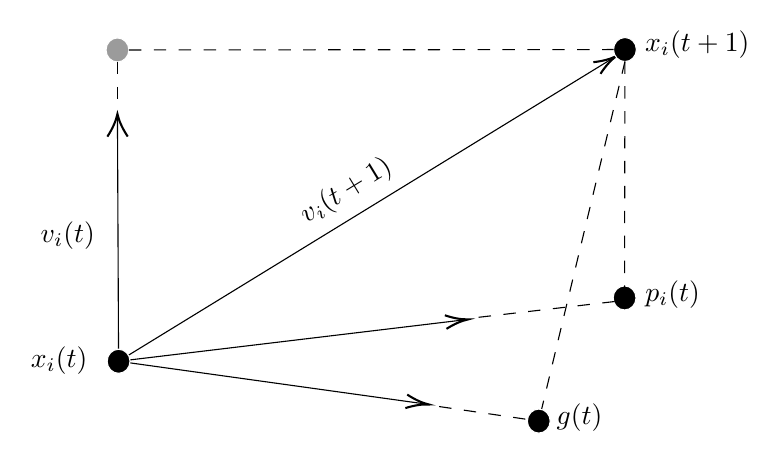
\begin{tikzpicture}[x=0.75pt,y=0.75pt,yscale=-1,xscale=1]
	\centering
	%uncomment if require: \path (0,429); %set diagram left start at 0, and has height of 429

	%Straight Lines [id:da4449765665231038]
	\draw    (90.55,300.19) -- (90.01,183) ;
	\draw [shift={(90,181)}, rotate = 449.73] [color={rgb, 255:red, 0; green, 0; blue, 0 }  ][line width=0.75]    (10.93,-4.9) .. controls (6.95,-2.3) and (3.31,-0.67) .. (0,0) .. controls (3.31,0.67) and (6.95,2.3) .. (10.93,4.9)   ;
	%Straight Lines [id:da7153141724618748]
	\draw [color={rgb, 255:red, 0; green, 0; blue, 0 }  ,draw opacity=1 ]   (90.55,300.19) -- (238.02,320.72) ;
	\draw [shift={(240,321)}, rotate = 187.93] [color={rgb, 255:red, 0; green, 0; blue, 0 }  ,draw opacity=1 ][line width=0.75]    (10.93,-3.29) .. controls (6.95,-1.4) and (3.31,-0.3) .. (0,0) .. controls (3.31,0.3) and (6.95,1.4) .. (10.93,3.29)   ;
	%Straight Lines [id:da049021320953235525]
	\draw [color={rgb, 255:red, 0; green, 0; blue, 0 }  ,draw opacity=1 ]   (90.55,300.19) -- (257.01,280.24) ;
	\draw [shift={(259,280)}, rotate = 533.1600000000001] [color={rgb, 255:red, 0; green, 0; blue, 0 }  ,draw opacity=1 ][line width=0.75]    (10.93,-3.29) .. controls (6.95,-1.4) and (3.31,-0.3) .. (0,0) .. controls (3.31,0.3) and (6.95,1.4) .. (10.93,3.29)   ;
	%Straight Lines [id:da20232334639948002]
	\draw [color={rgb, 255:red, 0; green, 0; blue, 0 }  ,draw opacity=1 ]   (90.55,300.19) -- (328.63,154.21) ;
	\draw [shift={(330.33,153.17)}, rotate = 508.48] [color={rgb, 255:red, 0; green, 0; blue, 0 }  ,draw opacity=1 ][line width=0.75]    (10.93,-3.29) .. controls (6.95,-1.4) and (3.31,-0.3) .. (0,0) .. controls (3.31,0.3) and (6.95,1.4) .. (10.93,3.29)   ;
	%Shape: Ellipse [id:dp2559339956288984]
	\draw  [color={rgb, 255:red, 255; green, 255; blue, 255 }  ,draw opacity=1 ][fill={rgb, 255:red, 155; green, 155; blue, 155 }  ,fill opacity=1 ] (84.49,150.2) .. controls (84.49,147) and (86.96,144.4) .. (90,144.4) .. controls (93.04,144.4) and (95.51,147) .. (95.51,150.2) .. controls (95.51,153.4) and (93.04,156) .. (90,156) .. controls (86.96,156) and (84.49,153.4) .. (84.49,150.2) -- cycle ;
	%Shape: Ellipse [id:dp6013524399579573]
	\draw  [color={rgb, 255:red, 255; green, 255; blue, 255 }  ,draw opacity=1 ][fill={rgb, 255:red, 0; green, 0; blue, 0 }  ,fill opacity=1 ] (85.04,300.19) .. controls (85.04,296.99) and (87.51,294.39) .. (90.55,294.39) .. controls (93.6,294.39) and (96.07,296.99) .. (96.07,300.19) .. controls (96.07,303.39) and (93.6,305.99) .. (90.55,305.99) .. controls (87.51,305.99) and (85.04,303.39) .. (85.04,300.19) -- cycle ;
	%Shape: Ellipse [id:dp34761974075621005]
	\draw  [color={rgb, 255:red, 255; green, 255; blue, 255 }  ,draw opacity=1 ][fill={rgb, 255:red, 0; green, 0; blue, 0 }  ,fill opacity=1 ] (329,150) .. controls (329,146.8) and (331.47,144.2) .. (334.51,144.2) .. controls (337.56,144.2) and (340.03,146.8) .. (340.03,150) .. controls (340.03,153.2) and (337.56,155.8) .. (334.51,155.8) .. controls (331.47,155.8) and (329,153.2) .. (329,150) -- cycle ;
	%Shape: Ellipse [id:dp8205390685372567]
	\draw  [color={rgb, 255:red, 255; green, 255; blue, 255 }  ,draw opacity=1 ][fill={rgb, 255:red, 0; green, 0; blue, 0 }  ,fill opacity=1 ] (328.82,269.67) .. controls (328.82,266.46) and (331.29,263.87) .. (334.33,263.87) .. controls (337.38,263.87) and (339.85,266.46) .. (339.85,269.67) .. controls (339.85,272.87) and (337.38,275.47) .. (334.33,275.47) .. controls (331.29,275.47) and (328.82,272.87) .. (328.82,269.67) -- cycle ;
	%Straight Lines [id:da9234883499988484]
	\draw  [dash pattern={on 4.5pt off 4.5pt}]  (95.51,150.2) -- (329,150) ;
	%Straight Lines [id:da37341255049105904]
	\draw  [dash pattern={on 4.5pt off 4.5pt}]  (90,156) -- (90,181) ;
	%Straight Lines [id:da30611169050284404]
	\draw [color={rgb, 255:red, 0; green, 0; blue, 0 }  ,draw opacity=1 ] [dash pattern={on 4.5pt off 4.5pt}]  (334.51,155.8) -- (293,329) ;
	%Straight Lines [id:da30982294243702113]
	\draw  [dash pattern={on 4.5pt off 4.5pt}]  (245,322) -- (293,329) ;
	%Shape: Ellipse [id:dp3097132743634232]
	\draw  [color={rgb, 255:red, 255; green, 255; blue, 255 }  ,draw opacity=1 ][fill={rgb, 255:red, 0; green, 0; blue, 0 }  ,fill opacity=1 ] (287.49,329) .. controls (287.49,325.8) and (289.96,323.2) .. (293,323.2) .. controls (296.04,323.2) and (298.51,325.8) .. (298.51,329) .. controls (298.51,332.2) and (296.04,334.8) .. (293,334.8) .. controls (289.96,334.8) and (287.49,332.2) .. (287.49,329) -- cycle ;
	%Straight Lines [id:da693045753345439]
	\draw  [dash pattern={on 4.5pt off 4.5pt}]  (264,279) -- (333,271) ;
	%Straight Lines [id:da6707373193501853]
	\draw  [dash pattern={on 4.5pt off 4.5pt}]  (334.33,269.67) -- (334.51,150) ;

	% Text Node
	\draw (51.74,231.56) node [anchor=north west][inner sep=0.75pt]    {$v_{i}( t)$};
	% Text Node
	\draw (174.1,224.92) node [anchor=north west][inner sep=0.75pt]  [rotate=-328.64]  {$v_{i}( t+1)$};
	% Text Node
	\draw (47.02,291.86) node [anchor=north west][inner sep=0.75pt]    {$x_{i}( t)$};
	% Text Node
	\draw (343,139.73) node [anchor=north west][inner sep=0.75pt]    {$x_{i}( t+1)$};
	% Text Node
	\draw (343.05,259.96) node [anchor=north west][inner sep=0.75pt]    {$p_{i}( t)$};
	% Text Node
	\draw (300.37,319.49) node [anchor=north west][inner sep=0.75pt]    {$g( t)$};
	\end{tikzpicture}
\end{figure}

	Алгоритм использует две последовательности равномерно распределенных случайных величин~$\xi_1(0), ..., \xi_1(t)$~и~$\xi_2(0), ..., \xi_2(t)$, которые масштабируются по константам~$c_1,\ c_2$. Данные константы влияют на максимальный размер шага, который частица может сделать за одну итерацию.	При~$c_1 = 0$~метод роения частиц будет опираться только на наилучшую позицию сообщества --- в таком случае алгоритм будет быстро сходиться, однако маловероятен факт нахождения глобального оптимума. При~$c_1 > 0$~метод использует связь всего сообщества --- скорость конвергенции падает, но глобальный оптимум оказывается более вероятным.

	\item Возвращаемся к 2 шагу, пока не достигнем оптимума.
\end{enumerate}

\subsection{Функция Розенброка}

\noindent
Функция Розенброка --- это невыпуклая функция вида
\[
	f(x, y) = (a - x)^2 + b(y-x^2)^2,
\]
использующаяся в качестве оценки производительности оптимизационных алоритмов. Она имеет глобальный минимум в точке $(a, a^2)$, где $f(a, a^2) = 0$.

Обычно $a = 1$, $b=100$. Тогда функция Розенброка примет следующий вид (рис. \ref{img:rosenbrock_0} и рис. \ref{img:rosenbrock_1}):
\[
	f(x, y) = (1 - x)^2 + 100(y-x^2)^2
\]

Глобальный минимум данной функции находится внутри <<долины>>: в нашем случае --- в точке $(1, 1)$. Найти долину достаточно легко, однако приблизиться к глобальному минимуму, считается, довольно сложно.

Только при $a = 0$, функция является симметричной, а ее минимум находится в начале координат.

\begin{figure}[ht]
	\centering
  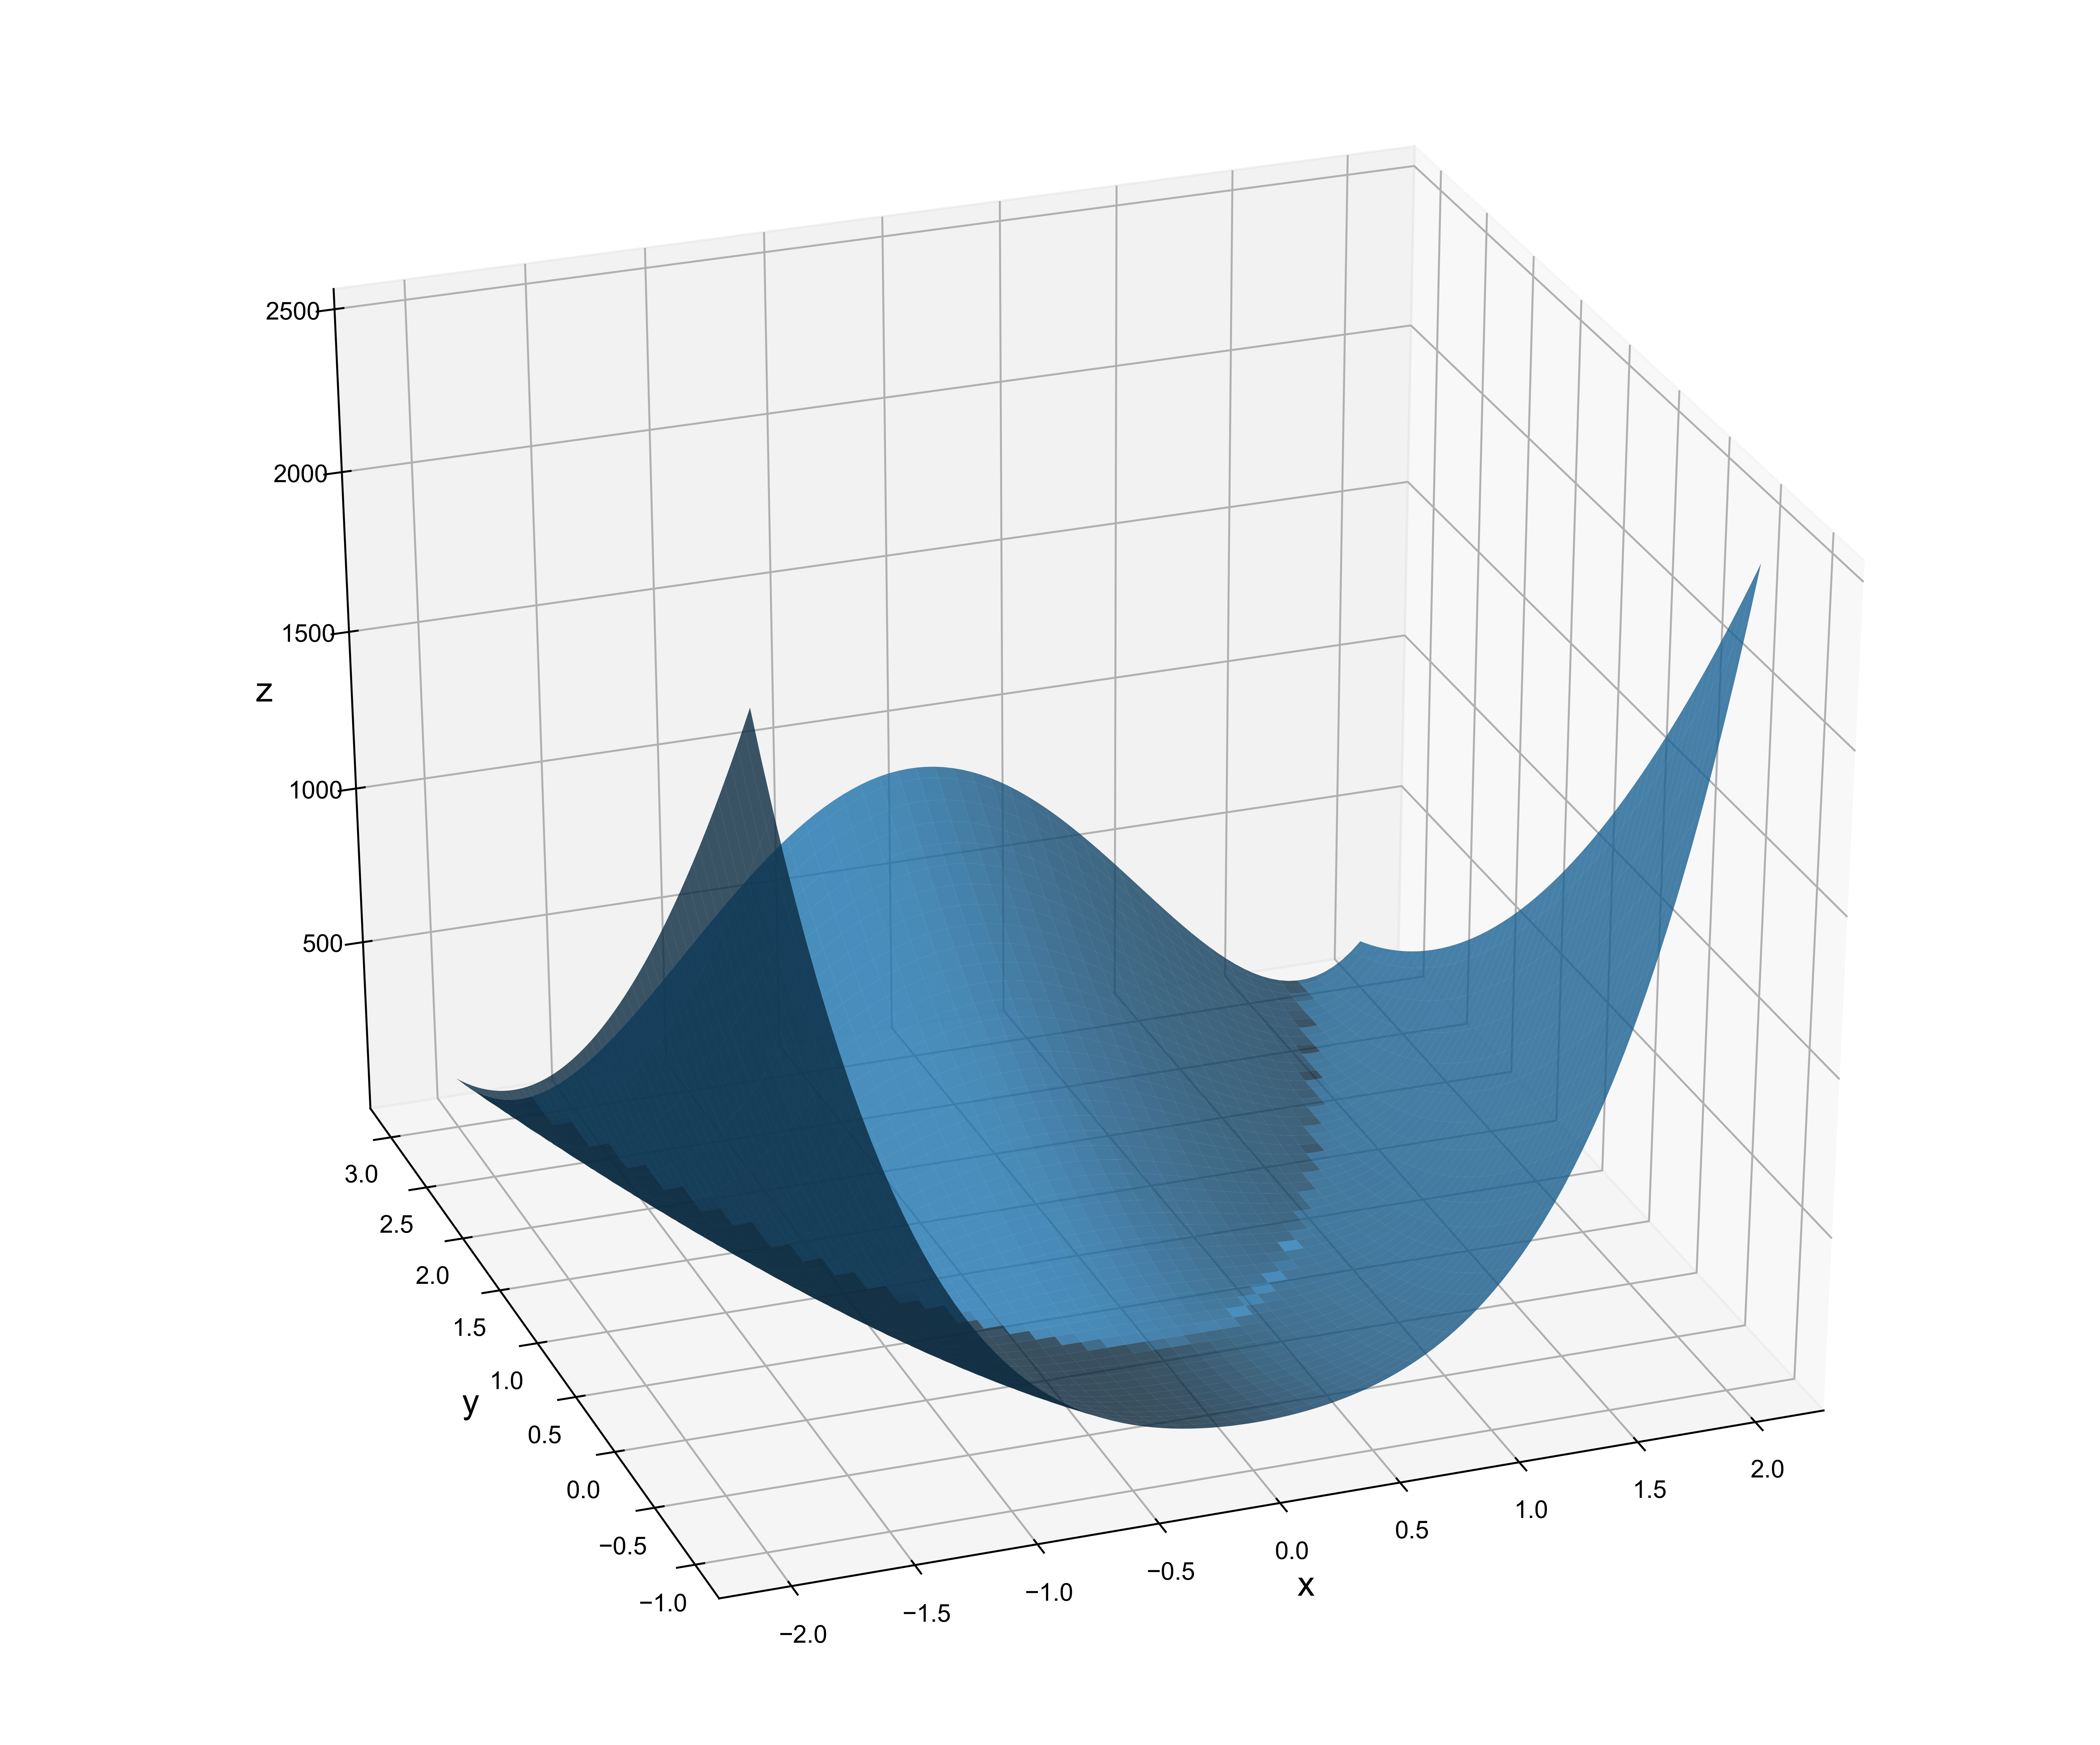
\includegraphics[width=120mm]{rosenbrock_0}
  \caption{ --- Функция Розенброка с параметрами $a = 1$, $b = 100$.}
  \label{img:rosenbrock_0}
\end{figure}

\newpage

\begin{figure}[ht]
	\centering
  \includegraphics[width=120mm]{rosenbrock_1}
  \caption{ --- Функция Розенброка с параметрами $a = 1$, $b = 100$.}
  \label{img:rosenbrock_1}
\end{figure}


Определим функцию Розенброка:
\begin{pyin}
def func(x):
  return (1 - x[0]) ** 2 + 100 * (x[1] - x[0] ** 2) ** 2
\end{pyin}

Инициализируем метод роения частиц, используя объектно-ориентированное программирование. В первую очередь cоздадим класс частиц.
\begin{pyin}
class Particle:
  def __init__(self, arg, space):
    self.pos = np.asarray([])      # расположение частицы
    self.velocity = np.asarray([]) # вектор скорости частицы
    self.pos_best = None           # лучшее расположение
    for i in range(arg):
       pos_i = np.random.uniform(space[i][0], space[i][1])
       self.pos = np.append(self.pos, pos_i)
       vel_i = np.random.uniform(0.2*space[i][0] , 0.2*space[i][1])
       self.velocity = np.append(self.velocity, vel_i)
    # pos_best --- это список, состоящий из лучшего расположения
    # частицы и значения функции в данной точке
    self.pos_best = [self.pos.copy(), func(self.pos)]

  def update_position(self):
    self.pos += self.velocity

  def update_velocity(self, w, c1, c2, swarm_best):
\end{pyin}



\begin{pyprint}
    inertion = w * self.velocity
    xi_1 = np.random.uniform()
    xi_2 = np.random.uniform()
    cognitive_acceler = c1 * xi_1 * (self.pos_best[0] - self.pos)
    social_acceler = c2 * xi_2 * (swarm_best - self.pos)
    self.velocity = inertion + cognitive_acceler + social_acceler

  def choose_personal_best(self):
    if func(self.pos) < func(self.pos_best[0]):
       self.pos_best[0] = self.pos.copy()
       self.pos_best[1] = func(self.pos)
\end{pyprint}

Теперь cоздадим класс ParticleSwarmOptimisation. Поскольку инерционный вес $w$ должен быть близким к $1$, а коэффициенты ускорения $c_1$, $c_2$ должны быть достаточно малыми, при инициализации класса установим гиперпараметры по умолчанию равными следующим величинам: $w=1.0$, $c1=0.2$, $c2=0.2$. Посредством метода search\_global будем искать глобальный минимум функции Розенброка.

\begin{pyin}
class ParticleSwarmOptimisation:
  def __init__(self, ell=40, w=1.0, c1=0.2, c2=0.2, max_iter=1000,
	       tol=1e-6):
    """
    PARAMETERS:
    ell --- количество частиц в рое.
    w --- инерционный вес.
    c1 --- коэффициент ускорения когнитивного воздействия на частицу.
    c2 --- коэффициент ускорения социального воздействия на частицу.
    max_iter --- максимальное количество итераций.
    tol --- точность.
    """
    self.ell = ell
    self.w = w
    self.c1 = c1
    self.c2 = c2
    self.max_iter = max_iter
    self.tol = tol
    self.swarm_best = None # лучшее расположение для всего роя
    self.swarm = None      # расположение всех частиц (рой)
\end{pyin}

\newpage
\begin{pyprint}
  def search_global(self, arg, space):
    """
    PARAMETERS:
    arg --- количество аргументов функции.
    space --- область поиска оптимума. Задается как список из
    кортежей, где кортеж --- это область значений
    одного аргумента функции.
    """
    self.arg = arg
    self.space = np.array(space)
    self.swarm = np.asarray([])

    # генерируем расположение роя
    for _ in range(self.ell):
       self.swarm = np.append(self.swarm,
                              Particle(self.arg, self.space))

    for k in range(self.max_iter):
       for i in range(self.ell):
          # обновляем расположение частицы
          self.swarm[i].update_position()
          # сравниваем с лучшей точкой частицы
          self.swarm[i].choose_personal_best()

       # выбираем лучшую точку для роя
       if k != 0:
          dist_0 = self.dist(self.swarm_best[0])
          self.choose_social_best()
          dist_1 = self.dist(self.swarm_best[0])

          # останавливаем поиск в условиях заданной точности
          if (dist_0 != dist_1) and (abs(dist_0-dist_1) <= self.tol):
             break
       else:
          self.choose_social_best()

       # обновляем вектор скорости
       for i in range(self.ell):
          self.swarm[i].update_velocity(self.w, self.c1,
                                        self.c2, self.swarm_best[0])

       print(f"Глобальный оптимум: {self.swarm_best[0]}")
       print(f"Значение функции в данной точке: {self.swarm_best[1]}")
\end{pyprint}

\begin{pyprint}
  def choose_social_best(self):
    best = min([[self.swarm[i].pos_best[0],
                 self.swarm[i].pos_best[1]] for i in range(self.ell)],
                 key=lambda x: x[1])
    self.swarm_best = best

  def dist(self, x):
    return np.sqrt(np.sum(x ** 2))
\end{pyprint}

\begin{figure}[h!]
\centering
\includegraphics[width=155mm]{swarm}
\caption{}
\label{img:swarm}
\end{figure}

Инициализируем рой c 100 частицами.
\begin{pyin}
sw = ParticleSwarmOptimisation(w=0.95, ell=100, tol=1e-20)
\end{pyin}

Отыщем глобальный минимум. Перемещение роя в поисках глобального оптимума представлено на рисунке \ref{img:swarm}.
\begin{pyin}
np.random.seed(53)
sw.search_global(2, [(-10, 10),(-10, 10)])
\end{pyin}

\begin{pyout}
Глобальный оптимум: [1. 1.].
Значение функции в данной точке: 6.366439023928984e-22.
\end{pyout}

Из графиков на рисунке \ref{img:PSO} видно, что за 1000 итераций метод роения частиц сходится к глобальному минимуму функции Розенборока с экспоненциальной скоростью с точностью 6.37e-22. Средняя скорость реализации алгоритма составляет 1.79 секунды со стандартным отклонением в 0.111 секунд.

\begin{figure}[ht]
  \begin{minipage}[ht]{0.49\linewidth}\centering
    \includegraphics[width=80mm]{PSO_2}
  \end{minipage}
  \hfill
  \begin{minipage}[ht]{0.49\linewidth}\centering
    \includegraphics[width=80mm]{PSO_3}
  \end{minipage}
  \caption{ --- Оптимизационный процесс.}
  \label{img:PSO}
\end{figure}
